% *********************************************************************
% © 2021-2022 Jeremy Sylvestre
%
% Permission is granted to copy, distribute and/or modify this document
% under the terms of the GNU Free Documentation License, Version 1.3 or
% any later version published by the Free Software Foundation; with no
% Invariant Sections, no Front-Cover Texts, and no Back-Cover Texts. A
% copy of the license is included in the appendix entitled “GNU Free
% Documentation License” that appears in the output document of this
% PreTeXt source code. All trademarks™ are the registered® marks of
% their respective owners.
%
% *********************************************************************

\newcommand*{\xmin}{-2}
\newcommand*{\xmax}{2}
\newcommand*{\ymin}{-0.5}
\newcommand*{\ymax}{4}
\newcommand*{\func}{\x * \x}

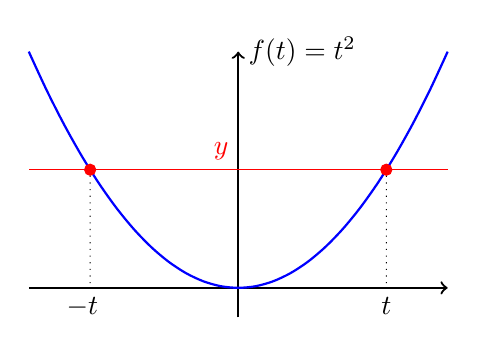
\begin{tikzpicture}
[
	closedpt/.style={circle,draw,fill,inner sep=0pt,minimum size=4pt},
	openpt/.style={circle,draw,inner sep=0pt,minimum size=4pt},
	xscale=1.33,
	yscale=0.75
]

	% axes
	\draw[->,thick] (\xmin,0) -- (\xmax,0); % node[below left] {$t$};
	\draw[->,thick] (0,\ymin) -- (0,\ymax) node[right] {$f(t) = t^2$};

	\draw[red] (\xmax,2) -- (\xmin,2);
	\node[red,above left] at (0,2) {$y$};

	% example graph
	\draw[thick, domain=\xmin:\xmax, smooth, blue] plot (\x,{\func});

	\node[closedpt,red] at (1.414,2) (pt) {};
	\draw[dotted] (pt) -- (1.414,0) node[below] {$t$};
	\node[closedpt,red] at (-1.414,2) (pt) {};
	\draw[dotted] (pt) -- (-1.414,0) node[below,xshift=-0.1cm] {$- t$};

\end{tikzpicture}
